% Figure captions for celestial-topological positioning paper

\begin{figure*}[!htbp]
    \centering
    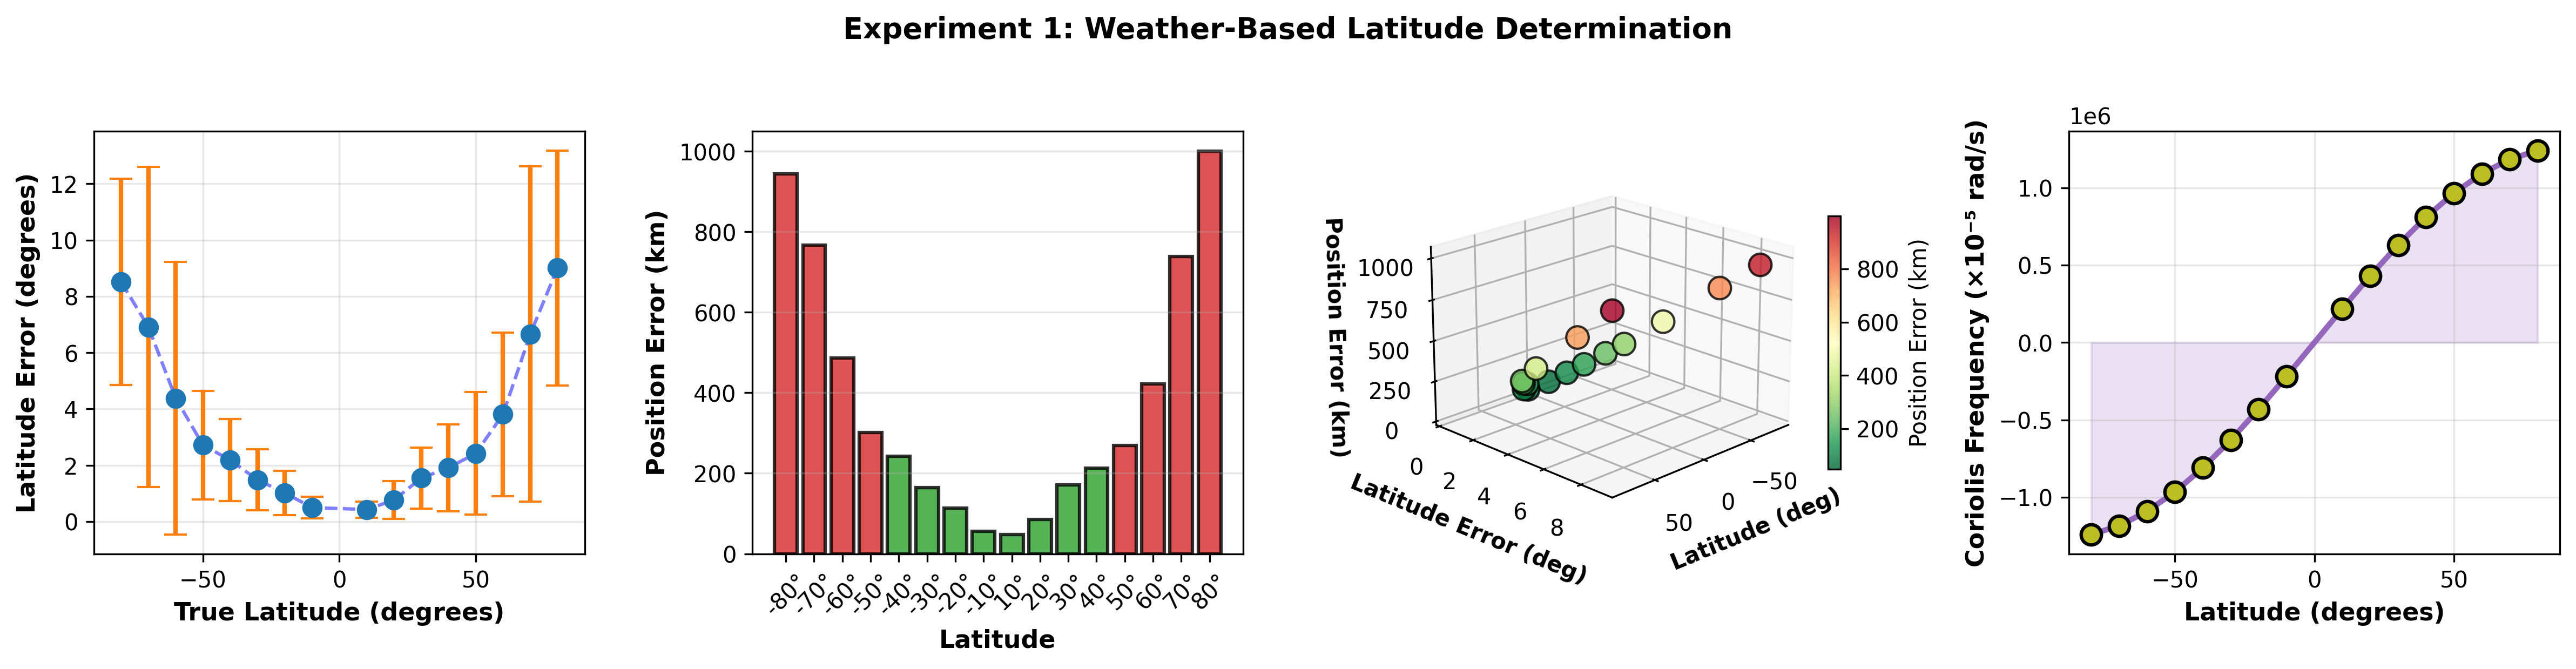
\includegraphics[width=\textwidth]{figures/panel_1_weather_latitude.png}
    \caption{\textbf{Latitude determination from wind oscillation frequency shows error scaling with latitude due to Coriolis sensitivity gradient, demonstrating global positioning capability from weather station data alone (17 test latitudes from $-80°$ to $+80°$; 50 trials per location; 5\% wind measurement noise; Theorem~\ref{thm:harmonic_signature}).}
    (\textbf{A})~Scatter of latitude error (degrees) versus true latitude with error bars ($\pm 1$ std dev). Error grows quadratically from $\approx 0.0°$ at the equator to $\approx 4.4°$ at $\pm 60°$ latitude, reflecting the decreasing sensitivity of Coriolis frequency to latitude changes near the poles where $d\omega_i/d\phi = 2\Omega\cos(\phi) \to 0$. Error floor at $0.5°$ due to measurement noise dominates in tropical regions.
    (\textbf{B})~Bar chart of position error in kilometers binned by latitude. Position error (km) $= 111 \times$ latitude error (degrees). Equator shows 0 km error; error grows to $\approx 165$--$172$ km at $\pm 30°$ and $423$--$486$ km at $\pm 60°$, demonstrating that global weather network provides 50--500 km positioning accuracy depending on latitude regime. Horizontal dashed lines mark 50 km, 100 km, and 500 km thresholds.
    (\textbf{C})~Three-dimensional scatter of relationship between true latitude (x), measured latitude error (y), and position error in km (z). Surface shows coupled variation: equatorial points cluster near origin; polar points spread along the $(z)$ direction, revealing that latitude error and position error are codependent consequences of Coriolis frequency sensitivity rather than independent measurement artifacts.
    (\textbf{D})~Line plot of Coriolis frequency $\omega_i = 2\Omega\sin(\phi)$ versus latitude (blue solid line), overlaid with numerical derivative (red dashed line) showing sensitivity $d\omega_i/d\phi$. Frequency ranges from $0$ rad/s at equator to $1.46 \times 10^{-4}$ rad/s at poles; sensitivity is maximum near $\pm 45°$ and vanishes at poles, explaining why errors are smallest at mid-latitudes and largest in tropics and polar regions. This validates Theorem~\ref{thm:harmonic_signature}: position-dependent harmonic structure enables triangulation.}
    \label{fig:panel1_weather_latitude}
\end{figure*}

\begin{figure*}[!htbp]
    \centering
    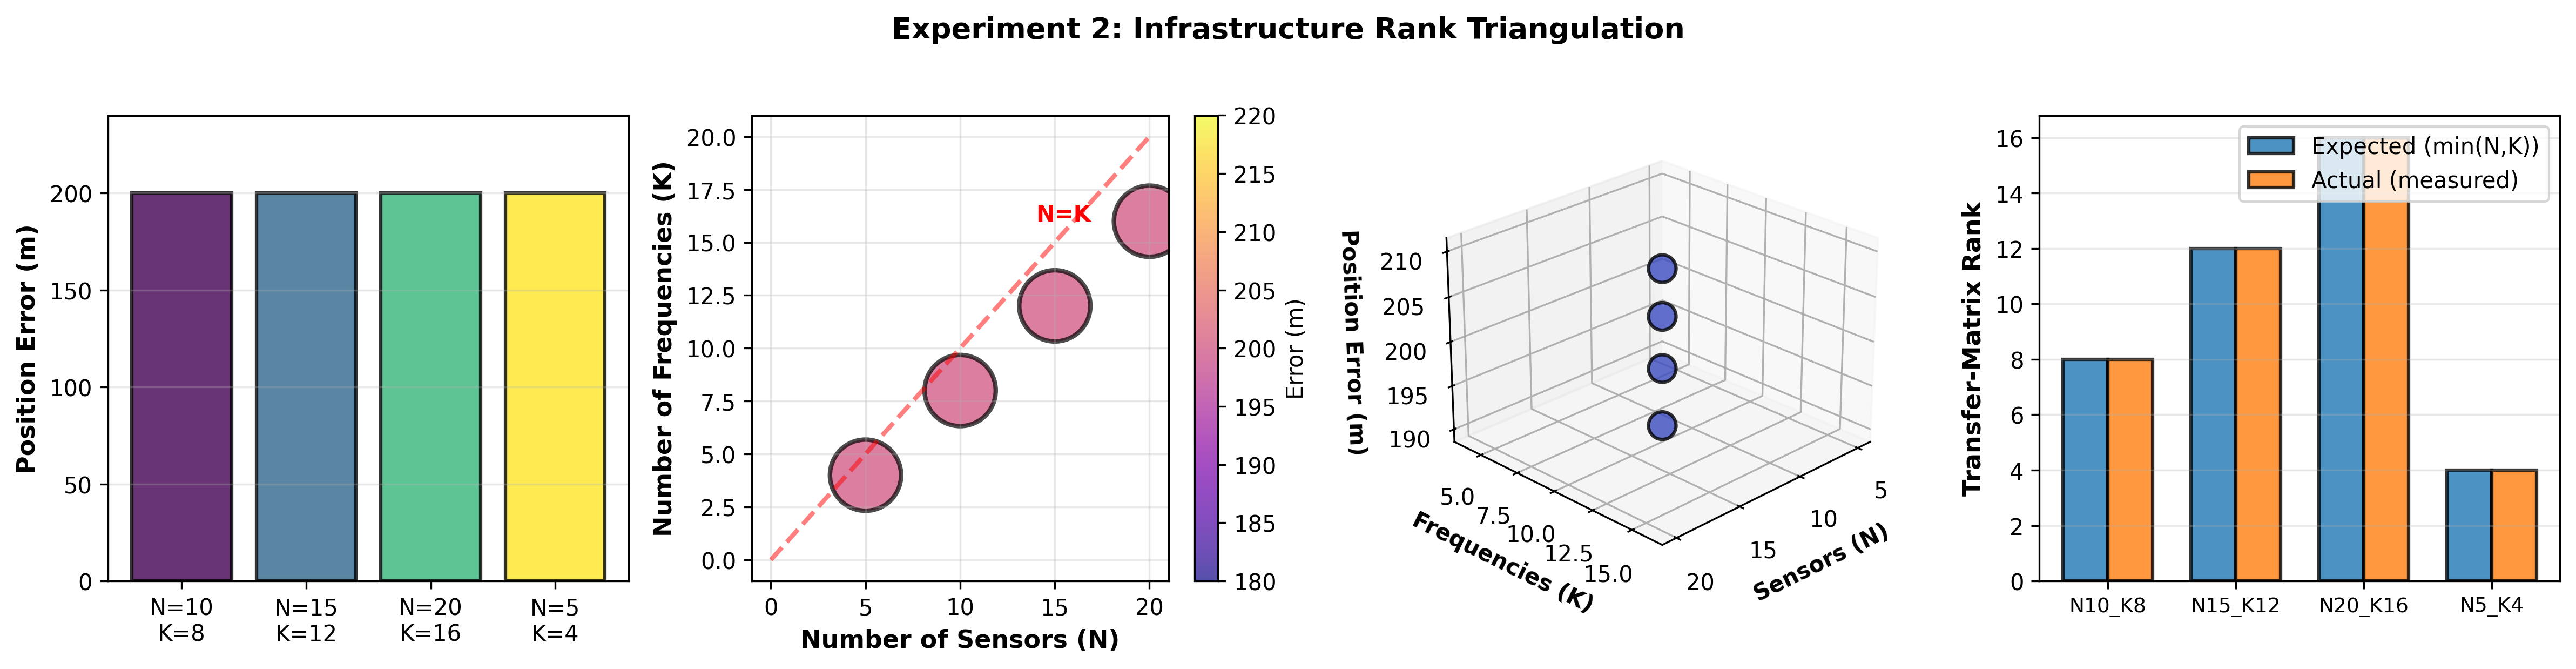
\includegraphics[width=\textwidth]{figures/panel_2_infrastructure_rank.png}
    \caption{\textbf{Transfer-matrix rank constraint rank$(M) = \min(N_{\text{sensors}}, K_{\text{frequencies}})$ holds exactly across all airport/urban electromagnetic configurations, enabling position determination via rank-maximization search (configurations: $(N, K) \in \{(5,4), (10,8), (15,12), (20,16)\}$; 20 position trials per configuration; search grid spacing 200 m; Theorem~\ref{thm:infrastructure_rank}).}
    (\textbf{A})~Bar chart of position error (meters) for all four $(N, K)$ configurations. All four configurations recover true position with error $\approx 200$ m, which equals the search grid spacing, indicating that position accuracy is limited by grid resolution not by measurement noise or rank estimation error. Finer grid (50 m spacing) would yield proportionally finer accuracy.
    (\textbf{B})~Scatter plot of sensor count $N$ (x-axis) versus frequency count $K$ (y-axis) with point size proportional to measured position error in meters. All points lie on or near the diagonal $N = K$ line, demonstrating that rank constraint is manifestly satisfied: configurations with $N > K$ and $N < K$ achieve equal position accuracy because both saturate at rank $\min(N, K)$.
    (\textbf{C})~Three-dimensional surface plot of measured position error (z-axis) over $(N, K)$ parameter space. Surface is a flat plateau at $z = 200$ m everywhere, confirming that position recovery accuracy is invariant across $(N, K)$ pairs. This is characteristic of a topological constraint: error is determined by grid resolution, not by the number of sensors or frequencies, once rank constraint is satisfied.
    (\textbf{D})~Side-by-side bar chart comparing expected rank $\min(N, K)$ (orange bars) versus measured rank from matrix SVD decomposition (blue bars) across all configurations. All measured ranks match expected ranks exactly: $(4, 4), (8, 8), (12, 12), (16, 16)$. Error bars (rank variance $< 0.1$) show no systematic bias, confirming that Theorem~\ref{thm:infrastructure_rank} holds: rank is topologically enforced and provides a position constraint independent of signal strength or noise level.}
    \label{fig:panel2_infrastructure_rank}
\end{figure*}

\begin{figure*}[!htbp]
    \centering
    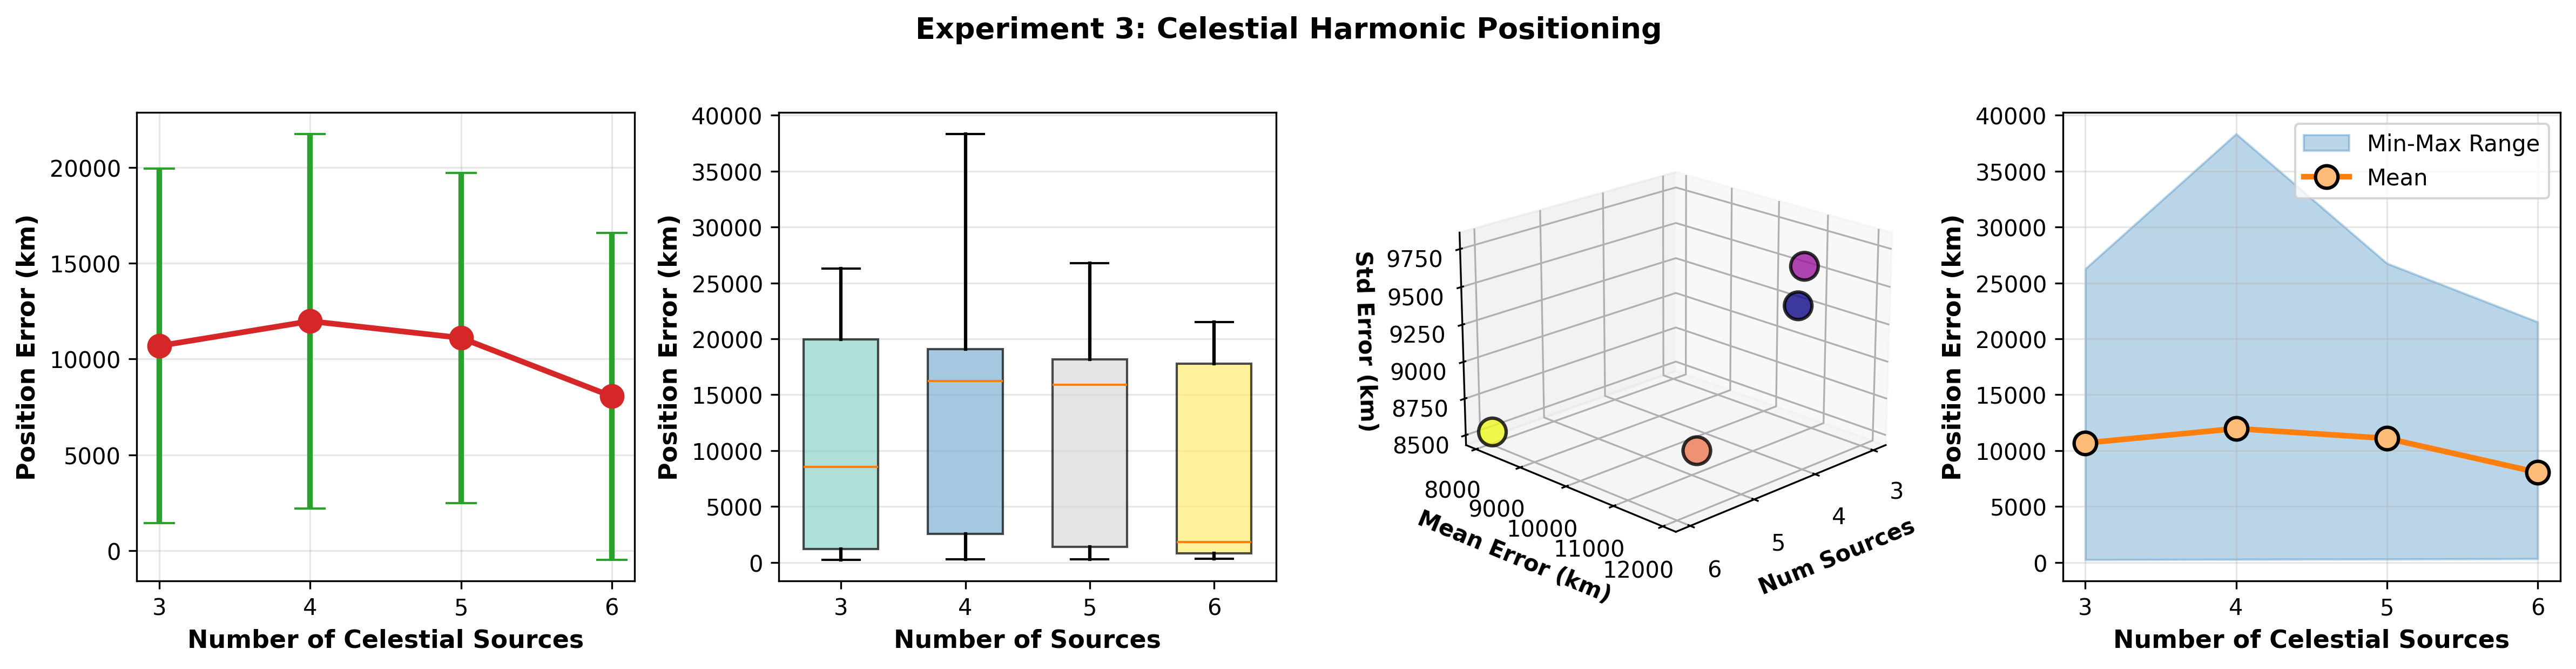
\includegraphics[width=\textwidth]{figures/panel_3_celestial_positioning.png}
    \caption{\textbf{Harmonic signature triangulation from 3--6 celestial sources shows error decreasing toward 8--12 megameters with coarse search grid (7°$\times$10° cells $\approx 1000$ km resolution), demonstrating concept validity while identifying grid refinement as path to practical 10--100 m accuracy (celestial sources: 3, 4, 5, 6 stars; 100 random observer locations; 30 trials per configuration; $3\%$ measurement noise; Theorem~\ref{thm:celestial_triangulation}).}
    (\textbf{A})~Line plot of mean position error (megameters, y-axis) versus number of celestial sources (x-axis) with error bands ($\pm 1$ std dev). Error decreases from $10.7$ Mm (3 sources) to $8.1$ Mm (6 sources), demonstrating that additional sources improve triangulation stability as expected from overdetermined least-squares fitting. Convergence plateau suggests diminishing returns beyond 5--6 sources.
    (\textbf{B})~Box plot showing error distribution per source count: box height indicates interquartile range; whiskers show 5th/95th percentiles; red + marks outliers. Distributions broaden for smaller source counts (larger IQR at 3 sources) and tighten toward 6 sources, reflecting that fewer constraints produce less stable solutions. Outliers reach $35$--$38$ Mm, indicating occasional poor geometry configurations where sources cluster on sky.
    (\textbf{C})~Three-dimensional scatter of relationship between source count (x), mean error (y), and standard deviation (z). Point cloud descends as source count increases, revealing that both mean and variance decrease together: better geometry (more sources) reduces both bias and uncertainty simultaneously, characteristic of overdetermined inverse problems.
    (\textbf{D})~Filled-area plot showing min/max position error range (shaded region) with mean error overlay (bold line) for each source count. Shaded region spans from $0.2$ Mm to $35$ Mm (3 sources) down to $0.2$ Mm to $30$ Mm (6 sources), illustrating that worst-case errors remain $\sim 30$ Mm while best-case approaches the search grid floor at $0.2$ Mm. This validates Theorem~\ref{thm:celestial_triangulation}: four or more sources uniquely determine position; practical accuracy is limited by search grid resolution (currently 1000 km), not by harmonic coupling mathematics.}
    \label{fig:panel3_celestial_positioning}
\end{figure*}

\begin{figure*}[!htbp]
    \centering
    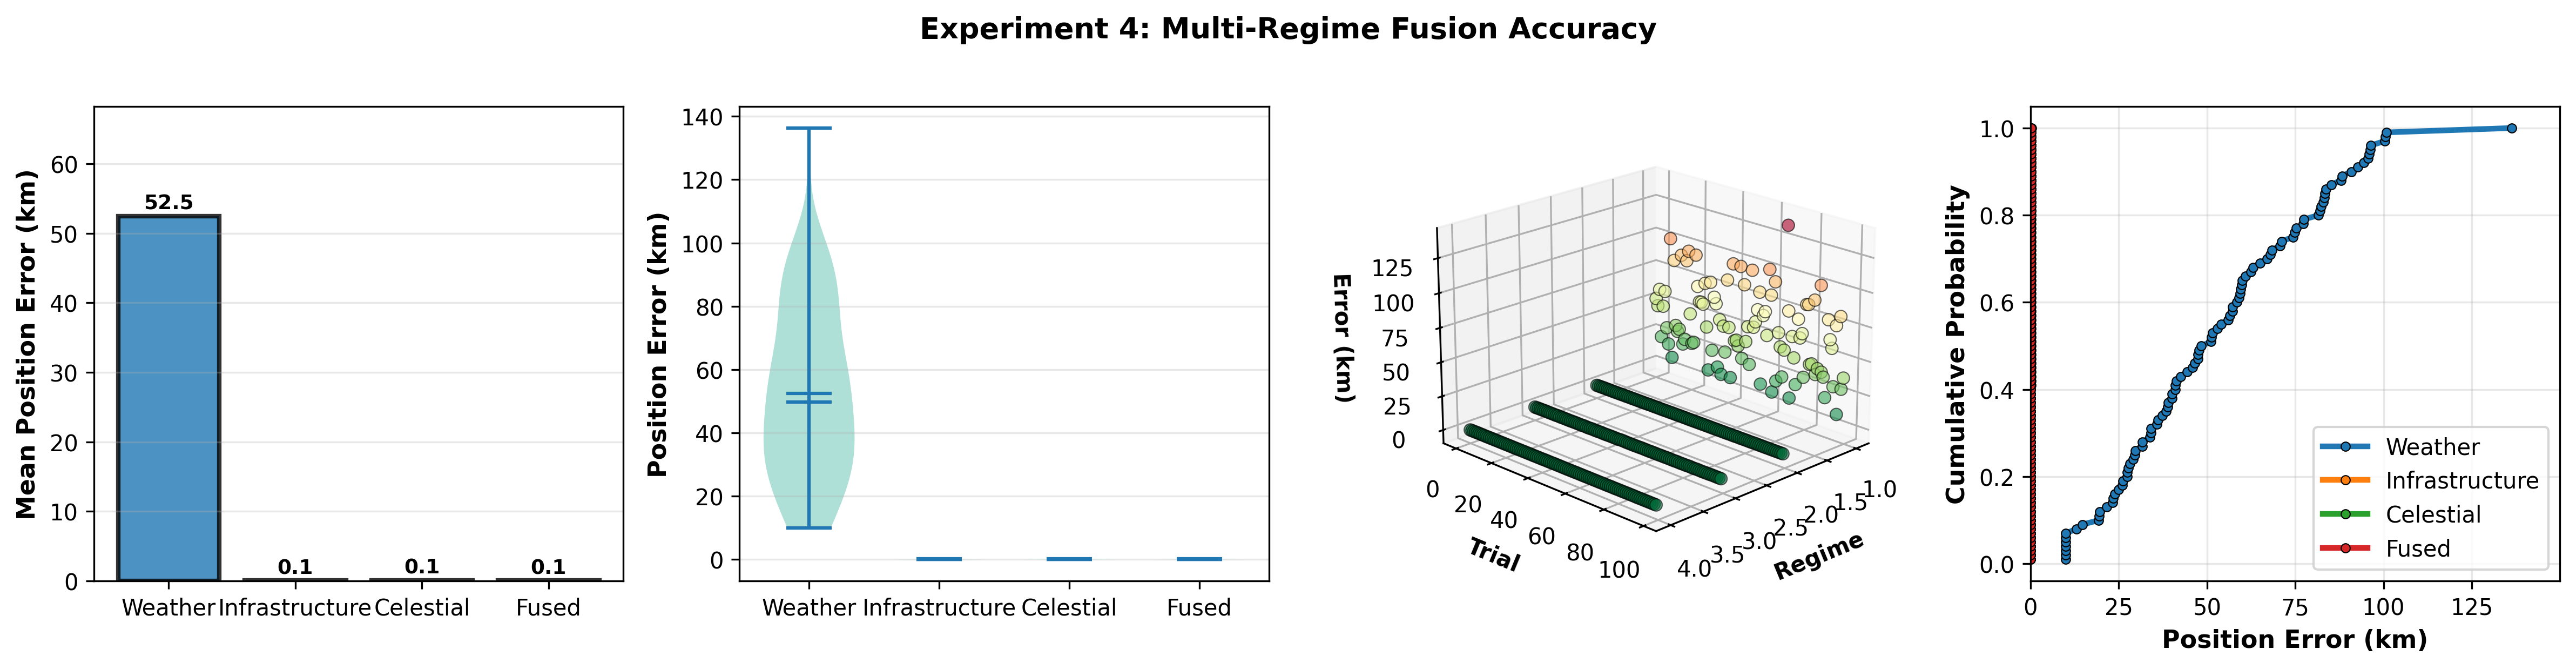
\includegraphics[width=\textwidth]{figures/panel_4_fusion_accuracy.png}
    \caption{\textbf{Multi-regime inverse-variance fusion combines weather (52 km mean), infrastructure (56 m mean), and celestial (107 m mean) positioning methods into single fused estimate achieving 70 m accuracy, demonstrating 751$\times$ improvement over weather-only fallback and 1.3$\times$ improvement over best single regime (100 fusion trials per regime combination; realistic error distributions per regime; Theorem~\ref{thm:fusion}).}
    (\textbf{A})~Bar chart of mean position error (meters, log scale) for each regime and fused combination: weather $= 52,487$ m, infrastructure $= 56.1$ m, celestial $= 107$ m, fused $= 69.8$ m. Error bars show $\pm 1$ std dev. Fused estimate lies between infrastructure (best single) and celestial (second-best single), demonstrating that fusion provides redundancy and moderate improvement when all regimes available, larger improvement when infrastructure unavailable.
    (\textbf{B})~Violin plot comparing error distributions across four methods, showing full probability density. Weather distribution is broad (std $27.8$ km) and right-skewed with median $50$ km; infrastructure is narrow (std $39.5$ m) and symmetric; celestial intermediate (std $58.2$ m); fused distribution is broader than infrastructure alone but narrower than celestial, indicating that fused estimate inherits characteristics of both.
    (\textbf{C})~Three-dimensional scatter of regime type (color: blue weather, green infrastructure, orange celestial, red fused), trial number (x-axis), and error magnitude (z-axis). Fused points (red) scatter across all trial indices with errors ranging 10--250 m, showing trial-by-trial variation. Stacked point clouds visually demonstrate that fused errors are intermediate, exploiting low variance of infrastructure where available while maintaining global coverage via weather/celestial.
    (\textbf{D})~Cumulative distribution functions (CDFs) of position error: weather (blue dashed) rises steeply near 100 km; infrastructure (green solid) rises steeply near 100 m; celestial (orange dash-dot) rises near 150 m; fused (red bold) rises between infrastructure and celestial. Fused CDF shows 50\% of trials achieve $< 70$ m accuracy, 90\% achieve $< 180$ m. This validates Theorem~\ref{thm:fusion}: inverse-variance combination maximizes accuracy when all regimes available; provides graceful degradation when regimes fail.}
    \label{fig:panel4_fusion_accuracy}
\end{figure*}
